% The data stencil of every part of a scheme name OWN-NEIGHBOUR/SPACE+TRANSITION, drawn.
% Plain TikZ, no extra package. The executable definition is sympy/scheme_matrix.py.
% Build: make scheme-stencils-figure
\documentclass[border=4pt]{standalone}
\usepackage[T1]{fontenc}
\usepackage{lmodern}
\usepackage{tikz}
\usetikzlibrary{calc}
\begin{document}
\sffamily
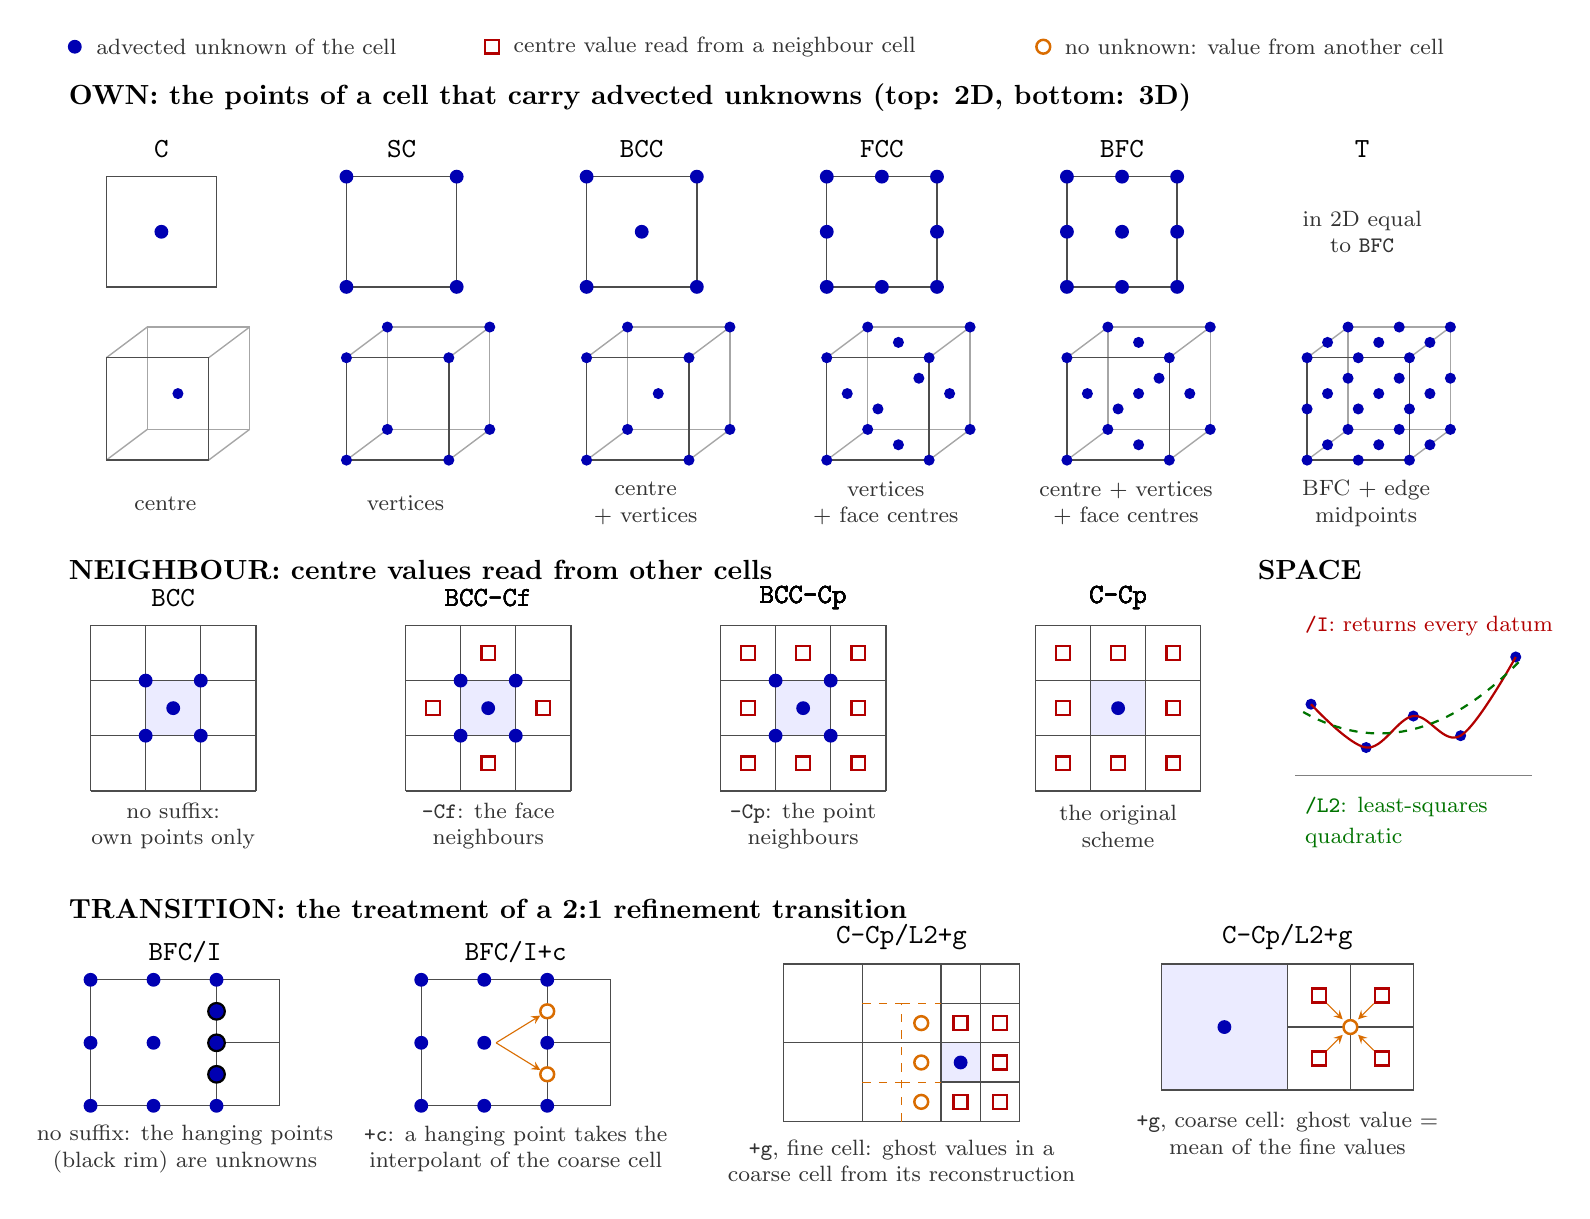
\begin{tikzpicture}[x=1cm, y=1cm, >=stealth,
    cell/.style={draw=black!70, line width=0.5pt},
    own/.style={circle, fill=blue!70!black, inner sep=0pt, minimum size=5pt},
    nbr/.style={rectangle, draw=red!70!black, line width=0.9pt, fill=white, inner sep=0pt, minimum size=5pt},
    gho/.style={circle, draw=orange!85!black, line width=0.9pt, fill=white, inner sep=0pt, minimum size=5pt},
    tok/.style={font=\ttfamily\bfseries},
    lab/.style={font=\footnotesize, align=center, text=black!80},
    row/.style={font=\bfseries, anchor=west}]
% ---------------------------------------------------------------- macros
% a unit square with lower left corner (#1,#2) and size #3; point sets
\newcommand{\sq}[3]{\draw[cell] (#1,#2) rectangle ++(#3,#3);}
\newcommand{\ptsC}[3]{\node[own] at (#1+#3/2,#2+#3/2) {};}
\newcommand{\ptsV}[3]{\foreach \a/\b in {0/0,1/0,0/1,1/1} \node[own] at (#1+\a*#3,#2+\b*#3) {};}
\newcommand{\ptsF}[3]{\foreach \a/\b in {.5/0,.5/1,0/.5,1/.5} \node[own] at (#1+\a*#3,#2+\b*#3) {};}
% an oblique cube with front lower left corner (#1,#2), size #3
\newcommand{\cubeP}[5]{($(#1,#2)+(#3*#5,#4*#5)+(0.42*0,0)$)}
\newcommand{\cube}[3]{%
  \draw[cell, black!35] (#1+0.4*#3,#2+0.3*#3) rectangle ++(#3,#3);
  \foreach \a/\b in {0/0,1/0,0/1,1/1} \draw[cell, black!35] (#1+\a*#3,#2+\b*#3) -- ++(0.4*#3,0.3*#3);
  \draw[cell] (#1,#2) rectangle ++(#3,#3);}
% a cube point: (#1,#2) corner, #3 size, (#4,#5,#6) in [0,1]^3 with depth #6
\newcommand{\cp}[6]{\node[own, minimum size=4pt] at (#1+#4*#3+0.4*#6*#3,#2+#5*#3+0.3*#6*#3) {};}
% ---------------------------------------------------------------- legend
\node[own] at (0.1,11.55) {}; \node[lab, anchor=west] at (0.25,11.55) {advected unknown of the cell};
\node[nbr] at (5.4,11.55) {}; \node[lab, anchor=west] at (5.55,11.55) {centre value read from a neighbour cell};
\node[gho] at (12.4,11.55) {}; \node[lab, anchor=west] at (12.55,11.55) {no unknown: value from another cell};
% ---------------------------------------------------------------- OWN, 2D
\node[row] at (-0.1,10.9) {OWN: the points of a cell that carry advected unknowns (top: 2D, bottom: 3D)};
\foreach \i/\n/\d in {0/C/centre, 1/SC/vertices, 2/BCC/centre\\+ vertices, 3/FCC/vertices\\+ face centres, 4/BFC/centre + vertices\\+ face centres, 5/T/BFC + edge\\midpoints} {
  \pgfmathsetmacro{\x}{0.5+3.05*\i}
  \node[tok] at (\x+0.7,10.25) {\n};
  \ifnum\i<5 \sq{\x}{8.5}{1.4} \fi
  \cube{\x}{6.3}{1.3}
  \node[lab] at (\x+0.75,5.75) {\d};
}
\ptsC{0.5}{8.5}{1.4}
\ptsV{3.55}{8.5}{1.4}
\ptsC{6.6}{8.5}{1.4} \ptsV{6.6}{8.5}{1.4}
\ptsV{9.65}{8.5}{1.4} \ptsF{9.65}{8.5}{1.4}
\ptsC{12.7}{8.5}{1.4} \ptsV{12.7}{8.5}{1.4} \ptsF{12.7}{8.5}{1.4}
\node[lab] at (16.45,9.2) {in 2D equal\\to \texttt{BFC}};
% 3D point sets
\newcommand{\cV}[1]{\foreach \a in {0,1} \foreach \b in {0,1} \foreach \c in {0,1} {\cp{#1}{6.3}{1.3}{\a}{\b}{\c}}}
\newcommand{\cC}[1]{\cp{#1}{6.3}{1.3}{.5}{.5}{.5}}
\newcommand{\cF}[1]{\foreach \a/\b/\c in {.5/.5/0,.5/.5/1,.5/0/.5,.5/1/.5,0/.5/.5,1/.5/.5} {\cp{#1}{6.3}{1.3}{\a}{\b}{\c}}}
\newcommand{\cE}[1]{\foreach \a/\b/\c in {.5/0/0,.5/1/0,.5/0/1,.5/1/1,0/.5/0,1/.5/0,0/.5/1,1/.5/1,0/0/.5,1/0/.5,0/1/.5,1/1/.5} {\cp{#1}{6.3}{1.3}{\a}{\b}{\c}}}
\cC{0.5} \cV{3.55} \cC{6.6} \cV{6.6} \cV{9.65} \cF{9.65} \cC{12.7} \cV{12.7} \cF{12.7}
\cC{15.75} \cV{15.75} \cF{15.75} \cE{15.75}
% ---------------------------------------------------------------- NEIGHBOUR
\node[row] at (-0.1,4.9) {NEIGHBOUR: centre values read from other cells};
\newcommand{\blk}[2]{% 3x3 block, lower left (#1,#2), cell size 0.7
  \fill[blue!8] (#1+0.7,#2+0.7) rectangle ++(0.7,0.7);
  \draw[cell] (#1,#2) grid[step=0.7] ++(2.1,2.1);}
\newcommand{\nb}[4]{\node[nbr] at (#1+0.35+0.7*#3,#2+0.35+0.7*#4) {};}
\begin{scope}[shift={(0.3,2.1)}]
  \draw[cell] (0,0) grid[step=0.7] (2.1,2.1); \fill[blue!8] (0.7,0.7) rectangle (1.4,1.4); \draw[cell] (0.7,0.7) rectangle (1.4,1.4);
  \ptsC{0.7}{0.7}{0.7} \ptsV{0.7}{0.7}{0.7}
  \node[tok] at (1.05,2.45) {BCC}; \node[lab] at (1.05,-0.45) {no suffix:\\own points only};
\end{scope}
\begin{scope}[shift={(4.3,2.1)}]
  \draw[cell] (0,0) grid[step=0.7] (2.1,2.1); \fill[blue!8] (0.7,0.7) rectangle (1.4,1.4); \draw[cell] (0.7,0.7) rectangle (1.4,1.4);
  \ptsC{0.7}{0.7}{0.7} \ptsV{0.7}{0.7}{0.7}
  \foreach \a/\b in {0/1,2/1,1/0,1/2} \nb{0}{0}{\a}{\b}
  \node[tok] at (1.05,2.45) {BCC-Cf}; \node[lab] at (1.05,-0.45) {\texttt{-Cf}: the face\\neighbours};
\end{scope}
\begin{scope}[shift={(8.3,2.1)}]
  \draw[cell] (0,0) grid[step=0.7] (2.1,2.1); \fill[blue!8] (0.7,0.7) rectangle (1.4,1.4); \draw[cell] (0.7,0.7) rectangle (1.4,1.4);
  \ptsC{0.7}{0.7}{0.7} \ptsV{0.7}{0.7}{0.7}
  \foreach \a/\b in {0/0,1/0,2/0,0/1,2/1,0/2,1/2,2/2} \nb{0}{0}{\a}{\b}
  \node[tok] at (1.05,2.45) {BCC-Cp}; \node[lab] at (1.05,-0.45) {\texttt{-Cp}: the point\\neighbours};
\end{scope}
\begin{scope}[shift={(12.3,2.1)}]
  \draw[cell] (0,0) grid[step=0.7] (2.1,2.1); \fill[blue!8] (0.7,0.7) rectangle (1.4,1.4); \draw[cell] (0.7,0.7) rectangle (1.4,1.4);
  \ptsC{0.7}{0.7}{0.7}
  \foreach \a/\b in {0/0,1/0,2/0,0/1,2/1,0/2,1/2,2/2} \nb{0}{0}{\a}{\b}
  \node[tok] at (1.05,2.45) {C-Cp}; \node[lab] at (1.05,-0.45) {the original\\scheme};
\end{scope}
% ---------------------------------------------------------------- SPACE
\begin{scope}[shift={(15.6,2.3)}]
  \node[row] at (-0.6,2.6) {SPACE};
  \draw[black!50] (0,0) -- (3.0,0);
  \foreach \x/\y in {0.2/0.9,0.9/0.35,1.5/0.75,2.1/0.5,2.8/1.5} \node[own, minimum size=4pt] at (\x,\y) {};
  \draw[red!70!black, line width=0.8pt] plot[smooth, tension=0.6] coordinates {(0.2,0.9) (0.9,0.35) (1.5,0.75) (2.1,0.5) (2.8,1.5)};
  \node[lab, text=red!70!black, anchor=west] at (0,1.9) {\texttt{/I}: returns every datum};
  \draw[green!45!black, line width=0.8pt, dashed] plot[domain=0.1:2.9, samples=30] (\x,{0.86-0.62*\x+0.29*\x*\x});
  \node[lab, text=green!45!black, anchor=west] at (0,-0.4) {\texttt{/L2}: least-squares};
  \node[lab, text=green!45!black, anchor=west] at (0,-0.8) {quadratic};
\end{scope}
% ---------------------------------------------------------------- TRANSITION
\node[row] at (-0.1,0.6) {TRANSITION: the treatment of a 2:1 refinement transition};
% coarse cell (size 1.6) and two fine cells (0.8)
\newcommand{\twoone}{\draw[cell] (0,0) rectangle (1.6,1.6); \draw[cell] (1.6,0) grid[step=0.8] (2.4,1.6); \draw[cell] (1.6,0) rectangle (2.4,1.6);}
\begin{scope}[shift={(0.3,-1.9)}]
  \twoone
  \node[own] at (0.8,0.8) {}; \foreach \a/\b in {0/0,1.6/0,0/1.6,1.6/1.6,0.8/0,0.8/1.6,0/0.8} \node[own] at (\a,\b) {};
  \foreach \a/\b in {1.6/0.8,1.6/0.4,1.6/1.2} \node[own, fill=blue!70!black, draw=black, line width=0.8pt, minimum size=6pt] at (\a,\b) {};
  \node[tok] at (1.2,1.95) {BFC/I}; \node[lab] at (1.2,-0.55) {no suffix: the hanging points\\(black rim) are unknowns};
\end{scope}
\begin{scope}[shift={(4.5,-1.9)}]
  \twoone
  \node[own] at (0.8,0.8) {}; \foreach \a/\b in {0/0,1.6/0,0/1.6,1.6/1.6,0.8/0,0.8/1.6,0/0.8,1.6/0.8} \node[own] at (\a,\b) {};
  \foreach \a/\b in {1.6/0.4,1.6/1.2} {\node[gho] (g) at (\a,\b) {}; \draw[->, orange!85!black] (0.95,0.8) -- (g);}
  \node[tok] at (1.2,1.95) {BFC/I+c}; \node[lab] at (1.2,-0.55) {\texttt{+c}: a hanging point takes the\\interpolant of the coarse cell};
\end{scope}
\begin{scope}[shift={(9.1,-2.1)}]
  % prolongation: a fine cell reads ghost fine cells inside the coarse cells
  \fill[blue!8] (2.0,0.5) rectangle (2.5,1.0);
  \draw[cell] (0,0) rectangle (2.0,2.0); \draw[cell] (0,1.0) -- (2.0,1.0); \draw[cell] (1.0,0) -- (1.0,2.0);
  \draw[cell] (2.0,0) grid[step=0.5] (3.0,2.0); \draw[cell] (2.0,0) rectangle (3.0,2.0);
  \draw[orange!85!black, dashed] (1.5,0) -- (1.5,1.5) (1.5,0.5) -- (2.0,0.5) (1.5,1.5) -- (2.0,1.5) (1.0,1.5) -- (1.5,1.5) (1.0,0.5) -- (1.5,0.5);
  \node[own] at (2.25,0.75) {};
  \foreach \a/\b in {2.25/0.25,2.75/0.25,2.75/0.75,2.25/1.25,2.75/1.25} \node[nbr] at (\a,\b) {};
  \foreach \a/\b in {1.75/0.25,1.75/0.75,1.75/1.25} \node[gho] at (\a,\b) {};
  \node[tok] at (1.5,2.35) {C-Cp/L2+g}; \node[lab] at (1.5,-0.5) {\texttt{+g}, fine cell: ghost values in a\\coarse cell from its reconstruction};
\end{scope}
\begin{scope}[shift={(13.9,-1.7)}]
  % restriction: the coarse cell reads the mean of the four fine values
  \fill[blue!8] (0,0) rectangle (1.6,1.6);
  \draw[cell] (0,0) rectangle (1.6,1.6); \draw[cell] (1.6,0) grid[step=0.8] (3.2,1.6); \draw[cell] (1.6,0) rectangle (3.2,1.6);
  \node[own] at (0.8,0.8) {}; \node[gho] (m) at (2.4,0.8) {};
  \foreach \a/\b in {2.0/0.4,2.8/0.4,2.0/1.2,2.8/1.2} {\node[nbr] (f) at (\a,\b) {}; \draw[->, orange!85!black, shorten >=1pt] (f) -- (m);}
  \node[tok] at (1.6,1.95) {C-Cp/L2+g}; \node[lab] at (1.6,-0.55) {\texttt{+g}, coarse cell: ghost value =\\mean of the fine values};
\end{scope}
\end{tikzpicture}
\end{document}
